\documentclass[12pt]{article}

\usepackage{hcmus-report-template}
\usepackage{titlesec}

\setcounter{secnumdepth}{4}

\titleformat{\paragraph}
{\normalfont\normalsize\bfseries}{\theparagraph}{1em}{}
\titlespacing*{\paragraph}
{0pt}{3.25ex plus 1ex minus .2ex}{1.5ex plus .2ex}
% \usepackage{IEEEtran}
% \documentclass[conference]{IEEEtran}

% Disable indentation on new paragraphs
\setlength{\parindent}{0pt}

% Line spacing 1.5
\renewcommand{\baselinestretch}{1.5}

% Optional: graphic path
% \graphicspath{PATH_TO_GRAPHIC_FOLDER}

% To use Times font family, uncomment this row
% \usepackage{mathptmx}

% To use roman section / subsection, uncomment these rows
% \renewcommand{\thesection}{\Roman{section}}
% \renewcommand{\thesubsection}{\thesection.\Roman{subsection}}

% Define course name, report name and report title.
\newcommand{\coursename}{Nhập môn điện toán đám mây}
\newcommand{\reportname}{Intelligent Cloud-Based Log Analytics \& BI System}
\newcommand{\reporttitle}{Báo cáo đồ án 1}

\newcommand{\studentname}{
\begin{tabular}{l l} % Two columns: left-aligned
Nguyễn Minh Hiếu & 23120124 \\
Nguyễn Minh Tú & 23120101 \\
Nguyễn Xuân Duy & 23120121 \\

\end{tabular}
                        }


% Header
\lhead{\reportname}
\rhead{
University of Science, VNU-HCM\\
\coursename
}

% Footer
% \newcommand{\leftfooter}{\LaTeX\ by \href{https://github.com/trhgquan}{Quan, Tran Hoang}}
% \lfoot{\leftfooter}

% ============ DOCUMENT ============
\renewcommand\thesection{\Roman{section}}
\renewcommand\thesubsection{\arabic{subsection}}
\begin{document}

\pagenumbering{arabic}
\setcounter{page}{1}
% \pagenumbering{roman}
\begin{titlepage}
    \newcommand{\HRule}{\rule{\linewidth}{0.5mm}}
    \centering
    
    % University and department
    \textsc{\LARGE vietnam national university, ho chi minh city}\\[0.25cm]
    \textsc{\LARGE university of science}\\[0.25cm]
    \textsc{\LARGE faculty of information technology}\\[0.25cm]
    
    % Logo
    
\includegraphics[scale=.25]{img/hcmus-logo.png}
    
    % Center the title section
    \vspace*{\fill} % Pushes everything above up to fill space
    
    {
    \huge{\bfseries{\reporttitle}}\\[0.5cm]
    \Large{\bfseries{Topic: \reportname}}
    }\\[0.3cm]
    
    \vspace*{\fill} % Pushes everything below down to fill space
    
    % Course and student/teacher information
    \textbf{\large Course: \coursename}\\[0.5cm]
    
    \textit{Prepared by} \\
    \studentname
    \\[3 cm]
    % Date
    {\large \today}\\[1cm]
    
    \vfill
    \end{titlepage}
    

\tableofcontents
\pagebreak
% \listoftables
% \pagebreak
% \listoffigures
% \pagebreak


\section{Giới thiệu}

Đồ án này xây dựng hệ thống phân tích dữ liệu đám mây toàn diện cho một startup truyền thông, nhằm tối ưu hóa việc theo dõi hoạt động website và hành vi khách hàng.

Quy trình vận hành bắt đầu từ việc mô phỏng và truyền tải dữ liệu qua lớp thu nạp serverless, kết hợp AI để phân tích feedback người dùng. Toàn bộ dữ liệu được lưu trữ tại BigQuery, phục vụ việc huấn luyện mô hình dự báo (BigQuery ML) và trực quan hóa báo cáo trên Looker Studio.
\clearpage
\section{Kiến trúc hệ thống}


\clearpage
\section{Chi tiết triển khai}
\clearpage
\section{Kết quả}

\subsection{Thống kê tổng quan}

Sau khi chạy pipeline hoàn chỉnh với dữ liệu mô phỏng, hệ thống tạo ra các số liệu sau:

\begin{table}[H]
\centering
\begin{tabular}{|l|l|}
\hline
\textbf{Chỉ số} & \textbf{Giá trị} \\
\hline
Tổng số bản ghi xử lý & {\small 2504} \\
\hline
Bản ghi có feedback & {\small 771} \\
\hline
Điểm sentiment trung bình & {\small 0.01} \\
\hline
Tỷ lệ hành động mua hàng & {\small 24.9\%} \\
\hline
\end{tabular}
\caption{Thống kê tổng quan dữ liệu sau khi xử lý}
\end{table}

\subsection{Kết quả đánh giá mô hình BigQuery ML}

Mô hình logistic regression \texttt{purchase\_prediction} được huấn luyện trên dữ liệu đã làm giàu. Kết quả đánh giá mô hình sử dụng \texttt{ML.EVALUATE} như sau:

\begin{table}[H]
\centering
\begin{tabular}{|l|l|}
\hline
\textbf{Chỉ số Hiệu Năng} & \textbf{Giá trị} \\
\hline
Precision & {\small 0.0} \\
\hline
Recall & {\small 0.0} \\
\hline
Accuracy & {\small 0.758} \\
\hline
ROC AUC & {\small 0.552} \\
\hline
F1-Score & {\small 0.0} \\
\end{tabular}
\caption{Kết quả đánh giá mô hình dự đoán hành vi mua hàng}
\end{table}

Những chỉ số này phản ánh một thực tế quan trọng về tập dữ liệu đầu vào. Với mức ROC AUC chỉ đạt khoảng 0.55 và các chỉ số Precision/Recall ở mức thấp, mô hình hiện tại chưa thể phân loại chính xác hành vi mua hàng. Tuy nhiên, điều này cung cấp những insight kỹ thuật rất giá trị.

\subsection{Quan sát chính từ pipeline}

Từ quá trình triển khai và kết quả thu được, chúng em có những nhận xét sau:

\begin{enumerate}
    \item \textbf{Tính ổn định và hiệu năng của Data Pipeline}
    
    Trình mô phỏng tạo ra luồng sự kiện liên tục, Pub/Sub tiếp nhận và định tuyến không mất mát dữ liệu, và Cloud Function xử lý thành công từng tin nhắn.
    
    \item \textbf{Chất lượng dữ liệu và Giới hạn của Machine Learning}
    
    Sự sụt giảm hiệu năng của mô hình BQML là một minh chứng rõ nét cho nguyên lý "Garbage In, Garbage Out". Qua phân tích mã nguồn mô phỏng, các biến đầu vào (\texttt{response\_time\_ms}, \texttt{feedback}) và biến mục tiêu (\texttt{action}) được sinh ra hoàn toàn ngẫu nhiên và độc lập. Do không có mối tương quan logic thực tế nào tồn tại trong tập dữ liệu thô, thuật toán Logistic Regression không thể tìm ra quy luật phân loại. Điều này bài học lớn về việc chất lượng dữ liệu thu thập quyết định trực tiếp đến sự thành bại của mô hình AI.
    
    \item \textbf{Hiệu quả của công cụ trực quan hóa (Looker Studio)}
    
    Dashboard Looker Studio đã kết nối trực tiếp với BigQuery và cập nhật theo thời gian thực một cách hiệu quả, tiện lợi:
    \begin{itemize}
        \item Lưu lượng truy cập qua các khung giờ hoạt động của trình mô phỏng.
        \item Phân bố  của các hành động người dùng 
        \item Thống kê điểm số cảm xúc trung bình (sentiment gauge) toàn cục.
    \end{itemize}
    
    Việc tự động hóa báo cáo này giúp giảm thiểu thao tác thủ công và cung cấp cái nhìn trực quan ngay lập tức cho các bên liên quan.
\end{enumerate}

\subsection{Hình ảnh minh họa}

Dưới đây là các hình ảnh chính từ quá trình triển khai:

\begin{figure}[H]
    \centering
    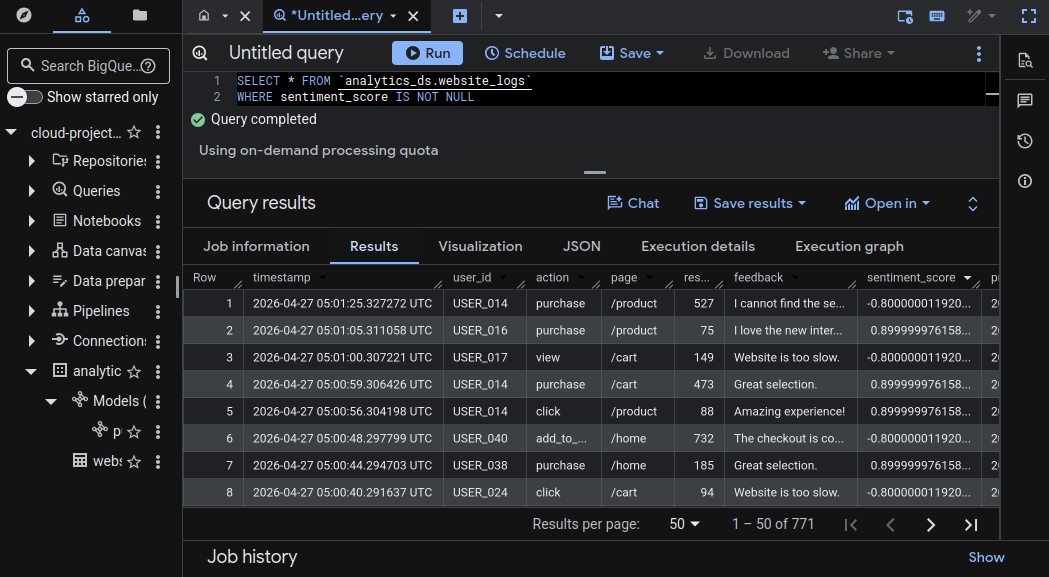
\includegraphics[width=0.85\textwidth]{img/result-bq-table.png}
    \caption{Bảng \texttt{website\_logs} trong BigQuery với các bản ghi đã xử lý và trường sentiment\_score}
\end{figure}

\begin{figure}[H]
    \centering
        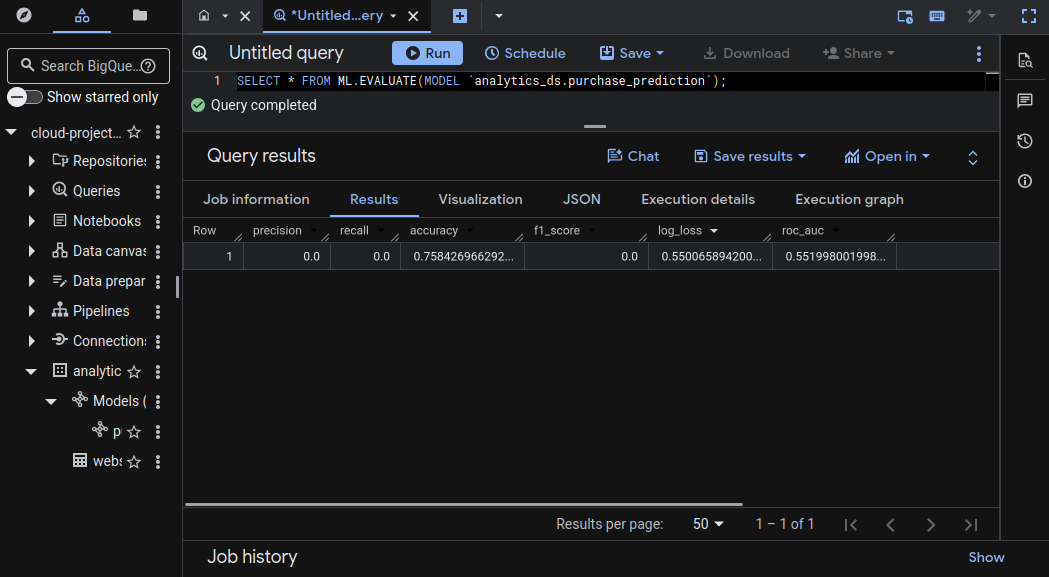
\includegraphics[width=0.85\textwidth]{img/result-bqml-evaluation.png}
        \caption{Kết quả đánh giá mô hình \texttt{purchase\_prediction} từ \texttt{ML.EVALUATE}}
\end{figure}

\begin{figure}[H]
    \centering
    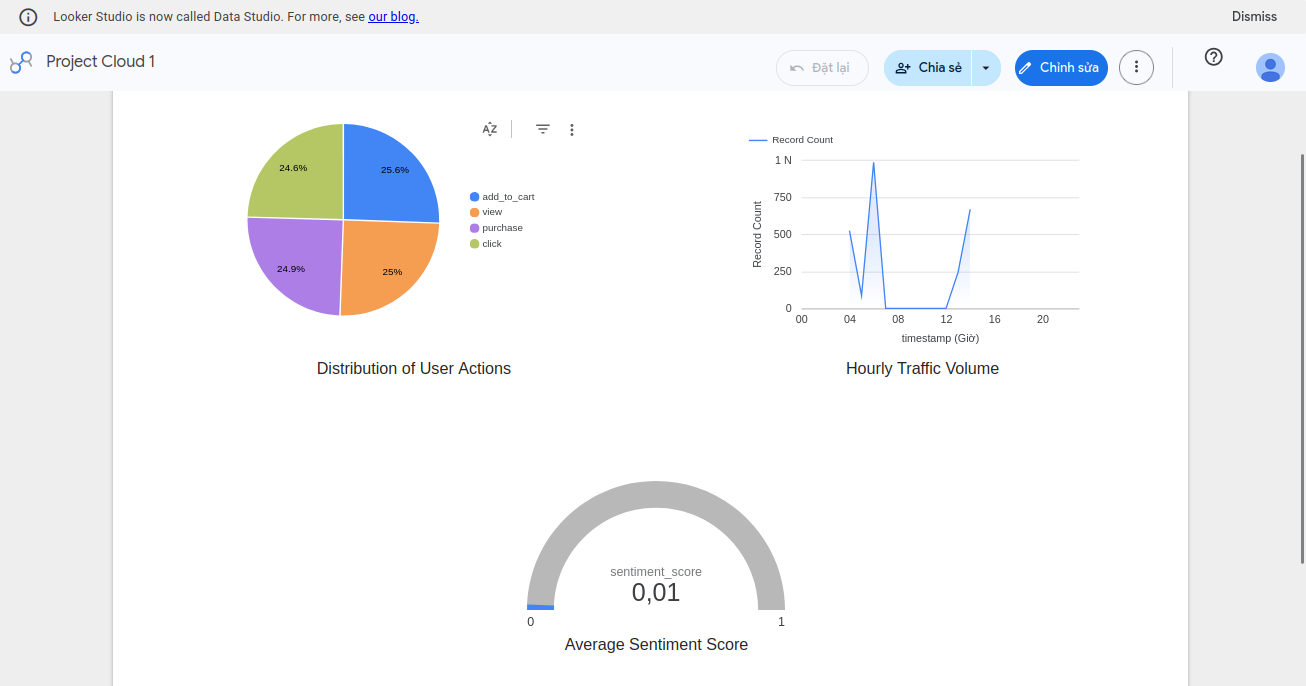
\includegraphics[width=0.9\textwidth]{img/phase-5-looker-dashboard.png}
    \caption{Dashboard Looker Studio hiển thị sentiment gauge, traffic time series, và action pie chart}
\end{figure}
\clearpage

% References
%\cleardoublepage
\phantomsection
\addcontentsline{toc}{section}{References}
\bibliographystyle{IEEEtran}
\nocite{*}
\bibliography{ref/ref.bib}


% Appendix
% \appendix
% Add \cleardoublepage to move appendices to next page.
%\input{appendix/appendix.tex}
\end{document}